\onehalfspacing
\section{Đề số 5}
\graphicspath{{./img/}}
\begin{bt} 
	\hfill
	\begin{enumerate}[a.]
		\item Tìm $x, y$ biết: $\frac{4+\mathrm{x}}{7+\mathrm{y}}=\frac{4}{7}$ và $\mathrm{x}+\mathrm{y}=22$
		\item Cho $\frac{x}{3}=\frac{y}{4}$ và $\frac{y}{5}=\frac{z}{6}$. Tính $M=\frac{2 x+3 y+4 z}{3 x+4 y+5 z}$
	\end{enumerate}
	\loigiai{
		\begin{enumerate}
			\item Ta có:
			$$
			\frac{4+x}{7+y} \Rightarrow 28+7 x=28+4 y \\ 
			\Rightarrow 7 x=4 y \\ 
			\Rightarrow \frac{x}{4}=\frac{y}{7}=\frac{x+y}{4+7}\\ 
		    \Rightarrow \frac{x}{4}=\frac{y}{7}=\frac{22}{11}=2 \\ 
			\Rightarrow x=8 ; y=14
			$$
			\item Ta có:\\ $$
			\begin{aligned}
				& \frac{x}{3}=\frac{y}{4} \Rightarrow \frac{x}{15}=\frac{y}{20} ; \frac{y}{5}=\frac{z}{6} \Rightarrow \frac{y}{20}=\frac{z}{24} \Rightarrow \frac{x}{15}=\frac{y}{20}=\frac{z}{24} \\
				& \text { (1) } \Rightarrow \frac{2 x}{30}=\frac{3 y}{60}=\frac{4 z}{96}=\frac{2 x+3 y+4 z}{30+60+96} \\
				& \text { (1) } \Rightarrow \frac{3 x}{45}=\frac{4 y}{80}=\frac{5 z}{120}=\frac{3 x+4 y+5 z}{45+80+120} \\
				& \Rightarrow \frac{2 x+3 y+4 z}{30+60+96}: \frac{3 x+4 y+5 z}{45+80+120}=\frac{2 x}{30}: \frac{3 x}{45} \\
				& \Rightarrow \frac{2 x+3 y+4 z}{186} \cdot \frac{245}{3 x+4 y+5 z}=1 \\
				&\Rightarrow M=\frac{2 x+3 y+4 z}{3 x+4 y+5 z}=\frac{186}{245}
				\end{aligned}$$
 		\end{enumerate}
	} 
\end{bt}

\begin{bt}
	Thực hiện tính:
	\begin{enumerate}[a.]
		\item $S=2^{2010}-2^{2009}-2^{2008} \ldots-2-1$
		\item $\mathrm{P}=1+\frac{1}{2}(1+2)+\frac{1}{3}(1+2+3)+\frac{1}{4}(1+2+3+4)+\ldots+\frac{1}{16}(1+2+3+\ldots+16)$
	\end{enumerate}
	\loigiai{
		\begin{enumerate}
			\item Ta có: $2 S=2^{2011}-2^{2010}-2^{2009} \ldots-2^2-2$
			$$
			\begin{aligned}
			& 2 \mathrm{~S}-\mathrm{S}=2^{2011}-2^{2010}-2^{2010} \cdot-2^{2009}+2^{2009} \cdot .-2^2+2^2-2+2+1 \\
			& \mathrm{~S} =2^{2011}-2 \cdot 2^{2010}+1 \\
			& \mathrm{~S} =2^{2011}-2^{2011}+1=1
			\end{aligned}
			$$
			\item Ta có:
			$$
			\begin{gathered}
			\mathrm{P}=1+\frac{1}{2} \cdot \frac{2 \cdot 3}{2}+\frac{1}{3} \cdot \frac{3 \cdot 4}{2}+\frac{1}{4} \frac{4 \cdot 5}{2}+\ldots+\frac{1}{16} \frac{16 \cdot 17}{2} \\
			=\frac{2}{2}+\frac{3}{2} \cdot+\frac{4}{2}+\frac{5}{2}+\ldots+\frac{17}{2} \\
			=\frac{1}{2}(1+2+3+\ldots+17-1) \\
			=\frac{1}{2}\left(\frac{17.18}{2}-1\right)=76
			\end{gathered}
			$$
		\end{enumerate}
	} 
\end{bt}

\begin{bt}
	Tìm x biết:
	\begin{enumerate}[a.]
		\item 
		 $\frac{1}{4} \cdot \frac{2}{6} \cdot \frac{3}{8} \cdot \frac{4}{10} \cdot \frac{5}{12} \ldots \frac{30}{62} \cdot \frac{31}{64}=2^{\mathrm{x}}$
		\item $\frac{4^5+4^5+4^5+4^5}{3^5+3^5+3^5} \cdot \frac{6^5+6^5+6^5+6^5+6^5+6^5}{2^5+2^5}=2^x$
	\end{enumerate}
	\loigiai{
		\begin{enumerate}
			\item Ta có:\\
			$ \frac{1}{2 \cdot 2} \cdot \frac{2}{2 \cdot 3} \cdot \frac{3}{2 \cdot 4} \cdot \frac{4}{2 \cdot 5} \cdot \frac{5}{2 \cdot 6} \cdots \frac{30}{2 \cdot 31} \cdot \frac{31}{2^6}=2^x \\
			\Leftrightarrow \frac{1 \cdot 2 \cdot 3 \cdot 4 \ldots 30.31}{1 \cdot 2 \cdot 3 \cdot 4 \ldots 30.31 \cdot 2^{30} \cdot 2^6}=2^x \\
			\Leftrightarrow \frac{1}{2^{36}}=2^x \\
			\Leftrightarrow x=-36$
			\item Ta có:	
			 $\frac{4.4^5}{3 \cdot 3^5} \cdot \frac{6 \cdot 6^5}{2 \cdot 2^5}=2^x \\
			 \Leftrightarrow \frac{4^6}{3^6} \cdot \frac{6^6}{2^6}=2^x\\ 
			 \Leftrightarrow  \left(\frac{6}{3}\right)^6 \cdot\left(\frac{4}{2}\right)^6=2^x \\
			 \Leftrightarrow2^{12}=2^x \\ 
			 \Rightarrow x=12$
		\end{enumerate}
	} 
\end{bt}

\begin{bt}
	Cho tam giác $A B C$ có $B<90^{\circ}$ và $B=2 C$. Kẻ đường cao $A H$. Trên tia đối của tia $B A$ lấy điểm $\mathrm{E}$ sao cho $\mathrm{BE}=\mathrm{BH}$. Đường thẳng $\mathrm{HE}$ cắt $\mathrm{AC}$ tại $\mathrm{D}$. 
	\begin{enumerate}[a.]
		\item Chứng minh $\mathrm{BEH}=\mathrm{ACB}$
		\item Chứng $\operatorname{minh} \mathrm{DH}=\mathrm{DC}=\mathrm{DA}$.
		\item Lấy $\mathrm{B}^{\prime}$ sao cho $\mathrm{H}$ là trung điểm của $\mathrm{BB}^{\prime}$. Chứng minh tam giác $\mathrm{AB}^{\prime} \mathrm{C}$ cân.
		\item Chứng minh $\mathrm{AE}=\mathrm{HC}$.
	\end{enumerate}
	\loigiai{
		$$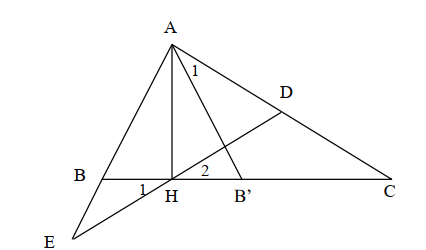
\includegraphics[width=0.55\textwidth]{5-4-lg.png}$$
		\begin{enumerate}
			\item $\mathrm{BEH}$ cân tại $\mathrm{B}$ nên $\widehat{E}=\widehat{\mathrm{H}_1}$\\
			$\widehat{A B C}=\widehat{E}+\widehat{\mathrm{H}_1}=2 \widehat{\mathrm{E}}$\\
			$\widehat{ABC}=2 \widehat{C} \Rightarrow \widehat{BEH}=\widehat{ACB}$
			\item Chứng tỏ được $\triangle \mathrm{DHC}$ cân tại $\mathrm{D}$ nên $\mathrm{DC}=\mathrm{DH}$.
			$\Delta \mathrm{DAH}$ có:
			$$
			\begin{gathered}
			\widehat{\mathrm{DAH}}=90^{\circ}-\mathrm{C} \\
			\widehat{DHA}=90^{\circ}-\widehat{\mathrm{H}_2}=90^{\circ}-\widehat{C}\\
			\Rightarrow \Delta \mathrm{DHA} \text { cân tại } \mathrm{D} \text { nên } \mathrm{DA}=\mathrm{DH} .
			\end{gathered}
			$$
			\item $\triangle \mathrm{ABB}^{\prime}$ cân tại $A$ nên $\widehat{\mathrm{B}^{\prime}}=\widehat{B}=2 \widehat{C}$\\
			$ \widehat{\mathrm{B}^{\prime}}=\widehat{A}_1+\widehat{C} \text { nên } 2 \widehat{C}=\widehat{A}_1+\widehat{C} \\
			 \Rightarrow \widehat{C}=\widehat{A}_1 \Rightarrow \widehat{{AB}^{\prime}C} \text { cân tại } \widehat{\mathrm{B}^{\prime}}$
			\item Ta có:\\
			$\mathrm{AB}=\mathrm{AB}^{\prime}=\mathrm{CB}^{\prime} \\
			\mathrm{BE}=\mathrm{BH}=\mathrm{B}^{\prime} \mathrm{H}
			\text { Có: } A E=A B+B E \\
			\mathrm{HC}=\mathrm{CB}^{\prime}+\mathrm{B}^{\prime} \mathrm{H} \\
			\Rightarrow \mathrm{AE}=\mathrm{HC}$
		\end{enumerate}
	}
\end{bt}